% This is samplepaper.tex, a sample chapter demonstrating the
% LLNCS macro package for Springer Computer Science proceedings;
% Version 2.20 of 2017/10/04
%
\documentclass[runningheads]{llncs}
%
\usepackage{graphicx}
% Used for displaying a sample figure. If possible, figure files should
% be included in EPS format.
%
% If you use the hyperref package, please uncomment the following line
% to display URLs in blue roman font according to Springer's eBook style:
% \renewcommand\UrlFont{\color{blue}\rmfamily}

\begin{document}
%
\title{ScSpark: Low-Redundancy disk access and High-Performance tool for the Single-Cell RNA sequenccing data processing\thanks{Supported by organization x.}}
%
%\titlerunning{Abbreviated paper title}
% If the paper title is too long for the running head, you can set
% an abbreviated paper title here
%
\author{First Author\inst{1}\orcidID{0000-1111-2222-3333} \and
Second Author\inst{2,3}\orcidID{1111-2222-3333-4444} \and
Third Author\inst{3}\orcidID{2222--3333-4444-5555}}
%
\authorrunning{F. Author et al.}
% First names are abbreviated in the running head.
% If there are more than two authors, 'et al.' is used.
%
\institute{Princeton University, Princeton NJ 08544, USA \and
Springer Heidelberg, Tiergartenstr. 17, 69121 Heidelberg, Germany
\email{lncs@springer.com}\\
\url{http://www.springer.com/gp/computer-science/lncs} \and
ABC Institute, Rupert-Karls-University Heidelberg, Heidelberg, Germany\\
\email{\{abc,lncs\}@uni-heidelberg.de}}
%
\maketitle              % typeset the header of the contribution
%
\begin{abstract}
High-throughout Single-cell RNA sequencing
  (scRNA-seq) data processing pipelines use multiple steps to transform raw scRNA-seq data to expression matrices, including record filtering, aligning and transcript counting.
Every two consecutive steps are connected by intermediate data.
However with the incresase of scRNA-seq data volume, file IO becomes the bottleneck of pipeline performance.
We take advantage of Spark's in-memory compute and scalable trait to develop a new Java-based program called ScSpark.
ScSpark can distribute single-cell RNA data processing tasks in the cluster and elminate all disk access for intermediate results.
Instead of the traditional way, we combine Spark and our proposed function to implement record filtering and transcript counting.
Furthermore, we choose STAR as our aligner.
In order to avoid unneccessary disk acess like extracted FASTQ file and SAM file, we use Java Native Interface(JNI) to deliver FASTQ RDD to STAR, and then transforms return value to SAM RDD.
We use pbmc\_10k\_v3 as our dataset and build spark's cluster on Aliyun to test ScSpark.
The experiment result shows indicates ScSpark faster and more scalable than any tradition pipeline.
\keywords{Intermediate Data \and Fast \and Scalable.}
\end{abstract}

\section{Introduction}

With the development of single-cell RNA sequencing (scRNA-seq) technology, it has become possible to perform large-scale transcript profifiling for tens of thousands of cells in a single experiment~\cite{gao2020Comparison}.
The large-scale single-cell sequencing technology represented by 10X Genomics platform is becoming the mainstream. 
The introduction of cellular barcodes (BC), sequences distinct for each cell attachted to the dT-primer, has increased the throughout and substantially reduced the cost of scRNA-seq.
These barcodes allow for the demultiplexing of reads after cells are pooled together for sequencing~\cite{tian2018scPipe}. 
Apart from cellular barcodes, Unique Molecular Identifiers (UMIs)\cite{Kivioja2012Counting}~\cite{camara2017Methods} are random oligonucleotide barcodes that are increasingly used in high-throughput sequencing experiments.
Through a UMI, identical copies arising from distinct molecules can be distinguished from those arising through PCR amplification of the same molecule~\cite{smith2017UMI}.
The multiple levels of barcoding uesd in scRNA-seq experiments create additional challenges in data processing, which is much different from RNA-seq and original scRNA-seq.
We won't discuss experiments where UMIs are not available, such as those conducted using non-barcoded scRNA-seq protocols.
Researchers around the world developed several scRNA-seq data processing pipelines typically implements multiple steps, including record filtering, aligning and transcript counting, to transform raw scRNA-seq data to expression matrices for further downstream analysis.
The first step is to filter Fastq reads that have low-quality BCs according to a user-defined threshold.
This step eliminates the majority of spurious BCs and thus greatly increase the accurate of BCs that need to be considered for counting, and simultaneously to filter low-quality UMIs.
The remaining Fastq reads are then mapping to the genome using the splice-aware aligner STAR~\cite{dobin2012RNA} or HISAT2~\cite{kim2015hisat}.
In ScSpark, we choose STAR as or aligner, which user is free to customize mapping by using the options.
Next, reads are assigned to genes and then generating count tables for UMIs and reads per gene per BC~\cite{swati0zUMIs}.

In a recently published article~\cite{gao2020Comparison}, they encapsulated seven existing
                                                                                          high-throughput
                                                                                                          scRNA-seq data processing pipelines with Nextflow, a general integrative workflow management framework, and evaluated their performances in terms of running time, computational resource consumption.
There are Drop-seq-tools~\cite{macosko2015Dropseq}, UMI-tools~\cite{smith2017UMI}, umis~\cite{macaulay0Svensson}, dropEst~\cite{viktor2018dropEst}, scPipe~\cite{tian2018scPipe}, zUMIs\cite{swati0zUMIs}, CellRanger\cite{zheng2017Massively}.
Among these pipelines, UMI-tools\cite{smith2017UMI} and CellRanger~\cite{zheng2017Massively} are the most representative.
UMI-tools~\cite{ref_url1} is an open source tool with an impressive clear process.
Unfortunately, all of the pipelines mentioned in this article run only on a single machine except CellRanger, and very slowly.
A big reason for these are the low level of parallelism.
To address this, STARsolo~\cite{2019STARsolo} has improved the parallelism of the mapping and counting process, and achieved good performance on a single machine.
However, it lacks filtering preprocessing and can't be extended to multiple nodes.
And CellRanger which is a highly integrated data process software tailored by 10X Genomics for single-cell RNA sequencing analysis and it go further in parallelism.
But the performance is lower than ScSpark and other parallelism pipeline that use big data tools.

There were many studies use big data framework like Apache Hadoop~\cite{ref_url2} and Apache Spark~\cite{ref_url3} to optimize biological data process.
Due to more efficiency in utilizing in memory computing, Spark is a better big data framework than Hadoop.
SparkBWA~\cite{abuin2016sparkbwa} and GPF~\cite{li2018high} are good framework that both solve DNA's upstream data process by using Apache Spark.
In the paper Falco~\cite{Yang2016Falco}, they are claimed to be a cloud-based framework to enable paralellization of existing RNA-seq processing pipelines using big data technologies of Hadoop and Spark for performing massively parallel analysis of large scale transcriptomic data. 
But Falco lack the filtering preprocessing due to the original pipeline has been transformed coarse-grained and their operations have lots of redundancy disk access which causes it doesn't utilize in memory compute advantage well.
It is safe to say that there is no scalable tool for transforming the entire scRNA-seq upstream data process pipeline with Spark.

\section{Method}
\subsection{Overview}
We implemented our program based on the Spark framework to utilize Spark's advantage, run program across the cluster, and default cache data keeps in memory.
With the increase of dataset volume, the time to process intermediate result file occupies a more significant proportion on total time.
And the single machine process capacity is not sufficient to adapt to the increasing scRNA-seq data volume.
Therefore, reducing the disk access of intermediate result file and improving the upstream data process's scalability is scSpark's primary target.

\subsection{Spark Version Filter}
\begin{figure}
  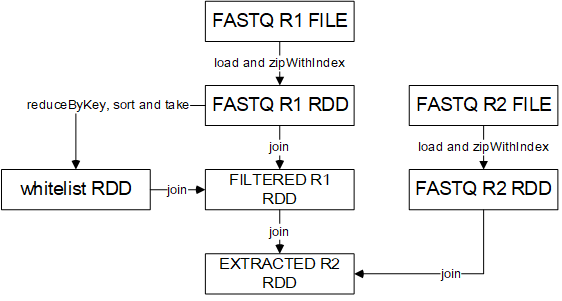
\includegraphics[width=\textwidth]{fig1.png}
  \caption{An overview of Spark version filter.} \label{fig1}
\end{figure}  
Our novelty Spark version filter aim to split large Fastq file to each node and take advantage of parallel computing.
Large FASTQ file can load in each node's memory parallel therefore the load speed doesn't limit by single node disk access speed.
As shown in Fig~\ref{fig1}, the filter step typically consists of two main components, generate whitelist which can identity of the true cell barcodes is unknown, use the whitelist to filter FASTQ R1 and then extract FASTQ R2 according to filtered FASTQ R1's index.

We load each split of FASTQ R1 to memory, and abstract them as FASTQ R1 RDD.
Generate whitelist actually is a top N problem that the problem can use Spark's function to achieve parllel compute.
By using reduceByKey function, FASTQ R1 RDD can count each split's barcodes times parallel and sum each split's result in the end.
After that we can use the result to generate whitelist RDD by Spark's sort and take function, both can parallel compute in the cluster.
We can easily get filtered FASTQ R1 RDD, by using the join function to find which read's cell barcode is in the whitelist.
The last step in filter is extracting FASTQ R2.
We use the join function again to combine filtered FASTQ R1 RDD and FASTQ R2 RDD with the same index.
\subsection{Eleminate redundancy disk access in Aligner step}
\begin{figure}
  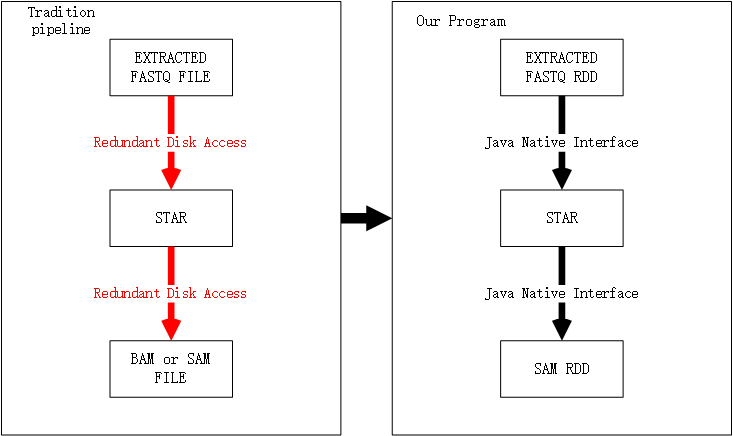
\includegraphics[width=\textwidth]{fig2.png}
  \caption{New way to implement STAR's interface.} \label{fig2}
\end{figure}
Apart from Cellranger we can't know how it implements because it isn't a open source software, in tradition pipeline, STAR need load extracted Fastq R2 file or load Fastq R1, R2 and whitelist actually will generate unneccessary disk access.  
We choose STAR as our aligner but modify how STAR loads FASTQ file to avoid load extracted FASTQ R2 and FASTQ R1 twice. 
As shown in Fig~\ref{fig2}, we utilize Java Native Interface to transfer extracted FASTQ R2 RDD's data to STAR, and then start the STAR process.
To overcome node's data volume imbalance problem, we repartition the extracted FASTQ R2 RDD, and then each node can run STAR parallel and with counterpoise data volume.
We also find if node's in memory is enough, we can start up more than one STAR's in one node to achieve better parallel.
STAR's result SAM or BAM file generate more disk access waste than STAR's input, we refer STAR-solo's solution to solve the problem by combining aligner and count.
We use Java Native Interface again to transfer STAR result and directly abstract them to SAM RDD.
This operation is parallel and totally in memory.

\subsection{Count with multi-node}
\begin{figure}
  \centering
  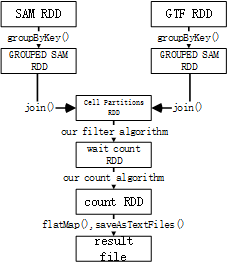
\includegraphics{fig3.png}
  \caption{An overview of Spark version count.} \label{fig3}
\end{figure}
As shown in Fig~\ref{fig3}, to take advantage multi-node's compute capability, we use a new way to implement count step.
Except SAM RDD that generate in the previous step, we load GTF file to memory and abstract them as GTF RDD.
Then we group SAM RDD and GTF RDD by their cell name and due to different cell's record can't influence the other's count, we use flatMap to parallel compute each cell's read count.
In the end, we collect result in all nodes, and the result file will produce the only output disk access in the whole program.
ScSpark breaks the limitation of one node's compute and can scale easily.

\section{Results}
We'll evaluate the speed, scalabilty and compare each step's scalability of our program in this section.
First, we'll run our program and tradition pipeline and use process time to evaluated the advantage of scSpark.
And then, the index of speedup helps us to examify the scalability of scSpark.
In the end, we compare each step's scalability to find the reason why scSpark's scalability also has a ceiling.
\subsection{Experiment environments and Data Sets prepare}
We use Apache Spark version 2.1.0 as our in-memory computing environment.
The Spark cluster consists of Aliyun's ECS, and each node consists of 16 vCPU
(Intel Xeon(Cascade Lake) Platinum 8269CY at 2.5GHz), 128 GBytes of DRAM and 400 GBits ESSD.

An example scRNA-seq dataset generated by 10X Genomics on their platform was used in our experiments.
10X-PBMC-10k dataset: 10X Genomics v3 10k peripheral blood mononuclear cell (PBMC) from a healthy donor~\cite{ref_url4}. 
It contains two gzipped FASTQ files, after unzip, FASTQ R1's volume is 69 Gbytes, and FASTQ R2's volume is 144 Gbytes, each of that file contain 640 millions records.
We used STAR as our aligner, mapping to an index built on the human NCBI38 reference which called GRCh38.p12.genome.fa and use genome.gtf~\cite{ref_url5} to filter the SAM~\cite{ref_url5}.
To evaluate the reason of why scSpark have a scalability ceiling and to experiment more convenient, we split FASTQ file to 100 millions, 160 millions and 320 millions records,.
\subsection{Performance Evaluation}
\begin{table}
  \centering
  \caption{tradition pipelien and scSpark's performance compare}\label{tab1}
  \begin{tabular}{l | l | l  l}
  \hline
  System &  Cores & Data volume size(s) \\
  \hline
   &  & 100 million(reads) & 640 million(reads) \\
  \hline
  UMI-tools & 64 cores & 7254 & 44160 \\
  \hline
  CellRanger & 64 cores & 6000 & 11700 \\
  \hline
  STAR-solo & 64 cores &  5820 & 8100 \\
  \hline
  scSpark & 4*16 cores & 354 & - \\
   & 8*16 cores & 210 & - \\
   & 16*16 cores & - & 841 \\
  \hline
  \end{tabular}
\end{table}
Limited by single machine's CPU cores, we only take 64 cores in traditional pipeline test as the traditional pipeline's performance.
Table~\ref{tab1} gives a summary of our program's performance and compare with tradition pipeline's performance.
We can see scSpark's speed is much more quick than any tradition pipeline in same CPU cores environment.
And scSpark can get improve when the cluster's CPU cores number increase.
\begin{table}
  \centering
  \caption{Each step performance compare}\label{tab2}
  \begin{tabular}{l | l | l | l | l}
  \hline
  System & Cores & filter & align & count \\
  \hline
  UMI-tools(100 million reads) & 64 cores & 9720 & 600 & 1740 \\
  \hline
  UMI-tools(640 million reads) & 64 cores & 33600 & 2160 & 8400 \\
  \hline
  scSpark(100 million reads) & 4*16 cores & 31 & 270 & 53 \\
  \hline
  scSpark(640 million reads) & 16*16 cores & 81 & 447 & 313 \\
  \hline
  \end{tabular}
\end{table}
Due to CellRanger isn't an open source software and STARsolo implements pipeline in a different way, we choose UMI-tools as scSpark each step's baseline.
As table~\ref{tab2} shown, scSpark is much faster than the traditional pipeline in any single step.
We can see the most significant improvement comes from the filter step because we make a traditional single thread operation to parallel computing in multi-machine and eliminate redundancy disk access.
For the same reason, scSpark's count step also gets considerable improvement.

\subsection{Scalability Evalution}
\begin{figure}
  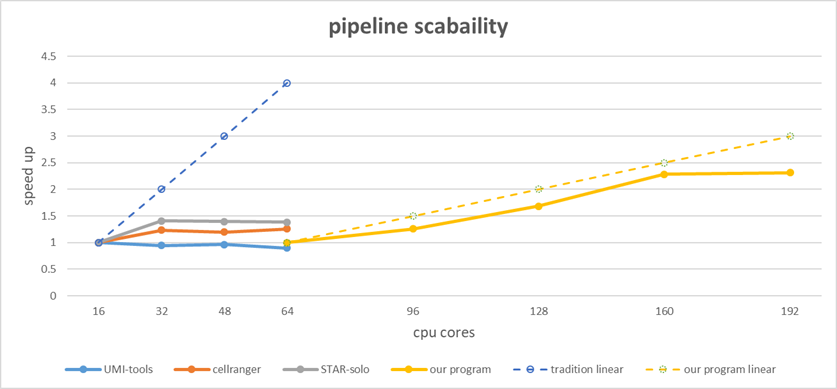
\includegraphics[width=\textwidth]{fig4.png}
  \caption{An overview of Spark version filter.} \label{fig4}
\end{figure}
ScSpark's second advantage is that it can get near linear improvement when the cluster's CPU core number improve.
To test the scalability of the tradition pipeline and scSpark, we use 16 CPU cores performance as tradition pipeline's baseline and 64 CPU cores performance as scSpark's baseline.
We use a small sample which have 100 millions records to compare speedup between our program and tradition pipeline.
As shown in Fig~\ref{fig5}, We found when CPU cores number increase our program can get near linear speedup and tradition pipeline's speedup far below linear speedup.
And we also found if the CPU cores number exceeds a ceiling, both tradition pipeline and scSpark will speedup nearly stop.
Umi-tools isn't showing any scalabiliy, even a little slow down when the CPU cores number increase.
STARsolo and CellRanger shows a little improve when the CPU cores increases to 32 from 16, but quickly stop speedup.
But scSpark ceiling is much higher than tradition pipeline.
All of it explain that our program more scalability than all tradition pipeline.
\subsection{Comparsion each step performance's increase}
\begin{figure}
  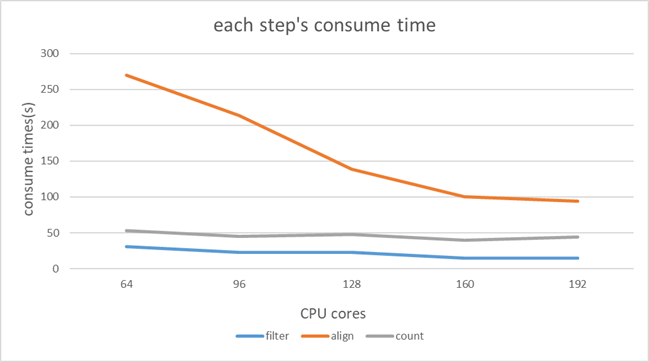
\includegraphics[width=\textwidth]{fig5.png}
  \caption{Each step consumes time.} \label{fig5}
\end{figure}
We also record each step's process time to know the reason of our improve and where can improve in future.
As shown in Fig~\ref{fig5}, we found our program's scalability most come from the align step and the align consumes most time in the whole program.
To find the reason why the align step is more scalability than the other step and why the scalability have a ceiling, we count how much records scSpark's STAR program can process.
We can find in Fig~\ref{fig6}, STAR's mapping speed is influenced by the data volume size and small volume dataset will lost its scalability earier than large volume dataset.
\begin{figure}
  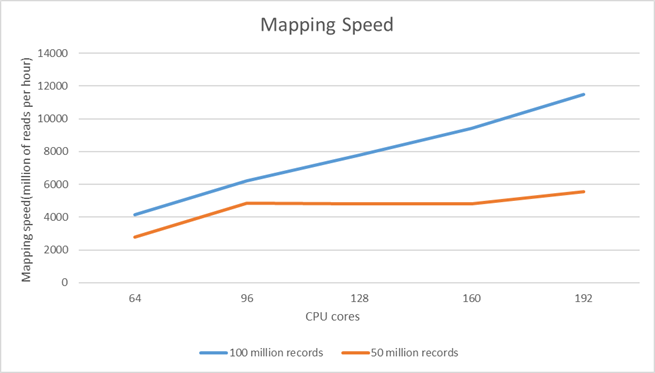
\includegraphics[width=\textwidth]{fig6.png}
  \caption{Each step consumes time.} \label{fig6}
\end{figure}

\begin{table}
  \centering
  \caption{Data volume influence}\label{tab3}
  \begin{tabular}{l | l | l | l | l}
  \hline
  Data volume(Million reads) & 10 & 50 & 100 & 640 \\
  \hline
  mapping speed(Million of reads per hour) & 250.28 & 503.83 & 503.02 & 950 \\
  \hline
  \end{tabular}
\end{table}

Then we test STAR program, and find the mapping speed is influenced by data volume.
As Table~\ref{tab3} shown, STAR mapping speed will increase when the data volume increase.
So when we get scalability by increase partition, each partition's read number decrease will limit the scalability increase.
\section{Conclusion}
In this paper, we propose a new way which utilize Apache Spark's in memory compute trait and we modify the filter and count, to speedup scRNA-seq upstream data process.
Our program can take advantage of multi machine compute capacity to speedup all step.
Modify filter and count algorithm to suit with parallel compute also get some improve.
Most important, eliminate redundant disk access can make our program much more quick than tradition pipeline.

Except performance improve, our program also show much more scalability than any tradition pipeline, and close to linear improve.
And we found our scalability is much come from align step.
Our program not only can imporve each partition process STAR program's mapping speed, but also can improve scalabliity by increasing partition number if the resource is sufficient.

But we also found scalability improve have a ceiling.
The reason is STAR program mapping speed influenced by loading index time, and if the data volume is small, the influence occupy a large proportion of whole STAR program process time.
We doubt if we can utilize distributed search~\cite{divya2013elasticsearch} or load index once in whole cluster to replace STAR, we can get more speedup and scalability.

Our next step work consists of two components.
First, we will use a new way to generate index and align by utilizing distributed search, to expand scalability.
Second, we think if we can change our program from batch process to stream process, we could reduce some waiting time between each continuous step.
\begin{thebibliography}{8}

%\bibliographystyle{splncs04}
%\bibliography{referenceTest}

\bibitem{gao2020Comparison}
Gao, M., Ling, M., Tang, X., Wang, S., Xiao, X., Qiao, Y., Yang, W., Yu, R.:
Comparison of high-throughput single-cell rna sequencing data processing
pipelines  (02 2020). \doi{10.1101/2020.02.09.940221}

\bibitem{tian2018scPipe}
Tian, L., Su, S., Dong, X., Amannzalcenstein, D., Biben, C., Seidi, A., Hilton,
D.J., Naik, S.H., Ritchie, M.E.: scpipe: A flexible r/bioconductor
preprocessing pipeline for single-cell rna-sequencing data. Plos One
\textbf{13}(7),  e0200193 (2018)

\bibitem{Kivioja2012Counting}
Kivioja, T., V?H?Rautio, A., Karlsson, K., Bonke, M., Enge, M., Linnarsson, S.,
Taipale, J.: Counting absolute numbers of molecules using unique molecular
identifiers. Nature Methods  \textbf{9}(1),  72--74 (2012)

\bibitem{camara2017Methods}
Camara, P.G.: Methods and challenges in the analysis of single-cell
rna-sequencing data. Current Opinion in Systems Biology  (2017)

\bibitem{smith2017UMI}
Smith, T., Heger, A., Sudbery, I.: Umi-tools: modeling sequencing errors in
unique molecular identifiers to improve quantification accuracy. Genome
research  \textbf{27}(3), ~491 (2017)

\bibitem{dobin2012RNA}
Dobin, A., Davis, C.A., Schlesinger, F.: Rna-star : ultrafast universal spliced
sequences aligner : Supplementary materials. Hgdownload  (2012)

\bibitem{kim2015hisat}
Kim, D., Langmead, B., Salzberg, S.L.: Hisat: a fast spliced aligner with low
memory requirements. Nature methods  \textbf{12}(4),  357--360 (2015)

\bibitem{swati0zUMIs}
Swati, P., Christoph, Z., Beate, V., Wolfgang, E., Ines, H.: zumis - a fast and
flexible pipeline to process rna sequencing data with umis. Gigaence (6), ~6

\bibitem{macosko2015Dropseq}
Macosko, E.Z., Basu, A., Satija, R., Nemesh, J., Shekhar, K., Goldman, M.,
Tirosh, I., Bialas, A.R., Kamitaki, N., Martersteck, E.M., Trombetta, J.J.,
Weitz, D.A., Sanes, J.R., Shalek, A.K., Regev, A., McCarroll, S.A.: Highly
parallel genome-wide expression profiling of individual cells using nanoliter
droplets. Cell  \textbf{161}(5),  1202—1214 (May 2015).
\doi{10.1016/j.cell.2015.05.002},
\url{https://europepmc.org/articles/PMC4481139}

\bibitem{macaulay0Svensson}
Svensson, V., Natarajan, K.N., Ly, L.H., Miragaia, R.J., Labalette, C.,
Macaulay, I.C., Cvejic, A., Teichmann, S.A.: Power analysis of single-cell
rna-sequencing experiments. Nature Methods

\bibitem{viktor2018dropEst}
Viktor, P., Jimin, G., Ninib, B., Nicolas, S., Scadden, D.T., Samsonova, M.G.,Kharchenko, P.V.: dropest: pipeline for accurate estimation of molecular
  counts in droplet-based single-cell rna-seq experiments. Genome Biology
\textbf{19}(1), ~78 (2018)

\bibitem{zheng2017Massively}
Zheng, G.X.Y., Terry, J.M., Belgrader, P., Ryvkin, P., Bent, Z.W., Wilson, R.,
Ziraldo, S.B., Wheeler, T.D., Mcdermott, G.P., Zhu, J.a.: Massively parallel
digital transcriptional profiling of single cells. Nature Communications
\textbf{8},  14049 (2017)

\bibitem{ref_url1}
UMI\_tools, \url{https://github.com/CGATOxford/UMI-tools}. Last accessed 30
Nov 2020

\bibitem{2019STARsolo}
Blibaum~A, W.J., A., D.: Starsolo: single-cell rna-seq analyses beyond gene
expression [version 1; not peer reviewed]. Genome Informatics  (2019)

\bibitem{ref_url2}
Apache Hadoop framework, \url{https://hadoop.apache.org}. Last accessed 30
Nov 2020

\bibitem{ref_url3}
Apache Spark framework, \url{https://spark.apache.org/}. Last accessed 30
Nov 2020

\bibitem{abuin2016sparkbwa}
Abu{\'\i}n, J.M., Pichel, J.C., Pena, T.F., Amigo, J.: Sparkbwa: speeding up
the alignment of high-throughput dna sequencing data. PloS one
\textbf{11}(5),  e0155461 (2016)

\bibitem{li2018high}
Li, X., Tan, G., Wang, B., Sun, N.: High-performance genomic analysis framework
with in-memory computing. ACM SIGPLAN Notices  \textbf{53}(1),  317--328
(2018)

\bibitem{Yang2016Falco}
Yang, A., Michael, T., Lin, P., Ho, J.W.K.: Falco: a quick and flexible
single-cell rna-seq processing framework on the cloud. Bioinformatics (5), ~5
(2016)

\bibitem{ref_url4}
10xgenomics, \url{https://support.10xgenomics.com}. Last accessed 30
Nov 2020

\bibitem{ref_url5}
Index and GTF file, \url{https://www.gencodegenes.org/human/releases.html}. Last accessed 30
Nov 2020

\bibitem{divya2013elasticsearch}
Divya, M.S., Goyal, S.K.: Elasticsearch: An advanced and quick search technique
  to handle voluminous data. Compusoft  \textbf{2}(6), ~171 (2013)

\end{thebibliography}
\end{document}
